\section{General Use Cases}
As a motivation of our work, we describe distinct scenarios where the proposed thesis may be useful:

%-----Total number of use cases: 9 (3 from WIMU, 2 from ReLOD(using MFKC), 1 from CEDAL, 1 from DBpediaSameAs + 2 from the whole thesis(Heloise and Platona)).
%----- WIMU
% In this section, we present three use-cases to show that our hypothesis works on the proposed tasks.

% \subsubsection{Data Quality in Link Repositories}

% The first use-case is about quality assurance in a link repository by re-applying link discovery algorithms on the stored links.
% This task concerns important steps of the Linked Data Lifecycle, in particular \textit{Data Interlinking} and \textit{Quality}.
% Link repositories contain sets of links that connect resources belonging to different datasets. 
% Unfortunately, the subject and the object URIs of a link often do not have metadata available, hence their Concise Bounded Descriptions (CBDs) are hard to obtain.
% In following figure, $(D_1,...,D_n|x)$ : $D_n$ represent the datasets and $x$ is the quantity of literals. 
% The \textbf{input} for our service in this use-case is $S$; the \textbf{output} is $\{(D_1,3),(D_2,1),(D_3,2)\}$, where $D1$ most likely defines $S$ due to the highest number of literal. 
% In the same way, the dataset that most likely defines $T$ is $D_4$ with 7 literals. 
% Once we have this information, the entire CBD of the two resources $S$ and $T$ can be extracted and a Link Discovery algorithm can check whether the \texttt{owl:sameAs} link among them should subsist.


% \begin{figure}[htb] 
% 	\centering
% 	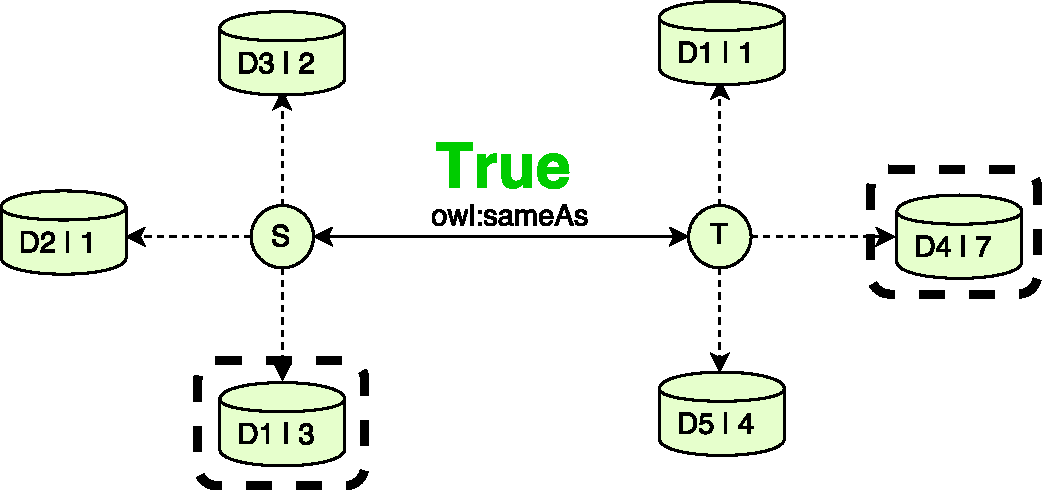
\includegraphics[width=250pt]{img/true.pdf}
% 	\label{fig:caseTrue}
% 	\caption{First use-case.}
% \end{figure}

% \subsubsection{Finding class axioms for Link Discovery}

% A class axiom is needed by the link discovery algorithm to reduce the number of comparisons. 
% Here, the aim is to find two class axioms for each mapping in the link repository.

% To this end, we use real data including a mapping\footnote{\url{http://www.linklion.org/download/mapping/citeseer.rkbexplorer.com---ibm.rkbexplorer.com.nt}} from the Link\-Lion repository~\cite{linklion2014} between \texttt{http://citeseer.rkbexplorer.com/id/resource-CS65161} ($S$) and \texttt{http://citeseer.rkbexplorer.com/id/resource-CS65161} ($T$). 
% Our service shows that $S$ was defined in four datasets, whereas the dataset with more literals was \url{http://km.aifb.kit.edu/projects/btc-2009/btc-2009-chunk-039.gz}\footnote{Also available in HDT file from \url{http://download.lodlaundromat.org/15b06d92ae660ffdcff9690c3d6f5185?type=hdt}}. 
% Thus, we can deduce where the URI $S$ was most likely defined.
% Knowing the datasets allows us to extract the axioms of the classes our URIs belong to.
% The techniques to decrease the complexity vary from choosing the most specific class to using an ontology learning tool such as DL-Learner~\cite{lehmann2009dl}.

% \begin{figure}[htb] 
% 	\centering
% 	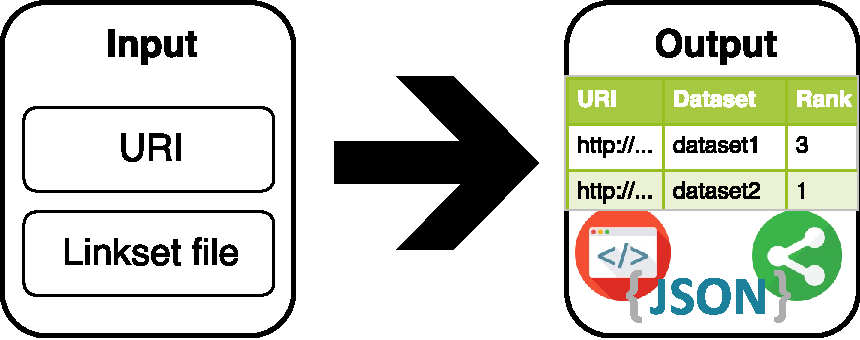
\includegraphics[width=150pt]{img/usage.pdf}
% 	\caption{Usage.}
% 	\label{fig:usage}
% \end{figure}

% \subsubsection{Federated Query Processing}
% Federated queries, which aim to collect information from more than one datasets is of central importance for many semantic web and linked data applications~\cite{saleem2013fostering,bigtcga2014}. One of the key step in federated query processing is the \emph{source selection}. The goal of the source selection is to find relevant sources (i.e., datasets) for the given user query. In the next step, the federated query processing engine makes use of the source selection information to generate an optimized query execution plan. WIMU can be used by the federated SPARQL engines to find the relevant sources against the individual triple patterns of the given SPARQL query. In particular, our service can be helpful during the source selection and query planning in cost-based SPARQL federation engines such SPLENDID~\cite{splendid2011}, SemaGrow~\cite{semagrow2015}, HiBISCuS~\cite{hibiscus2014}, CostFed~\cite{costfed2017}, etc. 

%----DBpediaSameAs
% \subsection{Normalization on DBpedia URIs}
% The criteria used in this evaluation are uniquely to tackle heterogeneity, that was observed during the search of co-references between different data sets with a problem about redundancies.

% When was used a URI from freebase in order to obtain a DBpedia URI was observed that at least 3 URIs were returned, that drives to the same final address.

% As an example of a real case, executed in our public server, with a URI from Freebase:

% \begin{lstlisting}
% $ curl http://dbpsa.aksw.org/SameAsService/SameAsServlet?uris=http%3A%2F%2Frdf.freebase.com%2Fns%2Fm.015fr

% returns: http://dbpedia.org/resource/Brazil
% \end{lstlisting}

% % \url{http://dbpsa.aksw.org/SameAsService/SameAsServlet?uris=http://rdf.freebase.com/ns/m.015fr}
% % returns: \url{http://dbpedia.org/resource/Brazil}

% Where, in this case, instead of 17 URIs from DBpedia, that goes to the same final address, our approach drives the user directly to the final address.

% As can be observed on the figure~\ref{fig:transient} that approach the transitive and redirect URIs, where show that with this approach instead of have several URIs the user can have only one from the DBpediaSameAs. Thus, in this way, providing a normalization on DBpedia URIs.

%-----CEDAL
% As our study case, we use a linkset repository called LinkLion~\cite{nentwig2014linklion} due to some advantages such as provenance, linksets from the most used datasets, i.e. DBpedia, Yago and Opencyc, where the users are empowered to upload links and specify how these were created. Moreover, users and applications can select and download sets of links via dumps or SPARQL queries. 

% The table \ref{tab:linkTypes} shows that $99.9 \%$ of links from LinkLion are \texttt{owl:sameAs} links, amounting to $19,200,114$ triples. Thus, in our experiments we are using only \texttt{owl:sameAs} links. 
% % All linkset files from LinkLion were copied locally to run the experiments.

% \begin{table}[H]
% 	\centering
% 	\caption{Link types}
% 	\label{tab:linkTypes}
% 	\begin{tabular}{ll}
% 		\hline\noalign{\smallskip}
% 		\textbf{Property}   & \textbf{Triples}  \\
% 		\noalign{\smallskip}
% 		\hline
% 		\textbf{sameAs}     & 19,606,657 (with duplicates)    \\
% 		\textbf{country}    & 1,309                 \\
% 		\textbf{author}     & 766              \\
% 		\textbf{spokenIn}   & 624                  \\
% 		\textbf{locatedIn}  & 250                  \\
% 		\textbf{exactMatch} & 167                 \\
% 		\textbf{near}       & 30                   \\
% 		\textbf{spatial\#P} & 28                   \\
% 		\textbf{seeAlso}    & 14             \\
% 		\textbf{organism}   & 14      \\
% 		\textbf{made}       & 4                \\
% 		\hline           
% 	\end{tabular}
% \end{table}
% %
% The experiments were performed using two configurations: (1) a laptop with Intel Core i7, 8 GB RAM, a video card NVIDIA NVS4200, Operational System MS Windows 10 and Java SE Development Kit 8. (2) An Intel Xeon Core i7 processor with 40 cores, 128 GB RAM on an Ubuntu 14.04.5 LTS with Java SE Development Kit 8. The results including the output file for LinkLion are available online.
% The total number of $19.6 million$ links was processed by our algorithm in $4.6$ minutes with the configuration (2). The total amount of errors were $1,352,366$ of candidates, where the total amount of domains were $254$ and  the number of linkset files was $553$, where $48.3\%$ of these knowledge base files has less than $10$ resources detected as erroneous candidates. 

% \subsubsection{Ranking the erroneous candidates}
% %Our ultimate goal is to detect links in \textit{large-scale link repositories}, resources sharing the same dataset.
% To evaluate how effective CEDAL is, we create a score in order to rank the erroneous candidates based on the number of detected resources with errors, in which the table \ref{tab:tuples}, show two fictional examples of tuples in the same pattern of the output from CEDAL.

% \begin{table}[H]
% 	\centering
% 	\caption{Fictional example results.}
% 	\label{tab:tuples}
% 	\begin{tabular}{@{}llll@{}}
% 		\toprule
% 		Knowledge-base & Data-set domain & \textbf{$\mathbb{C}$} & $\mu$ \\ \midrule
% 		Linkset1.nt                 & Data-set1         & URI1,URI2               & 1              \\
% 		Linkset2.nt                 & Data-set2         & {\small URI1,URI2,URI3,URI4}     & 6              \\ \bottomrule
% 	\end{tabular}
% \end{table}
% %
% The $\mu$ score is calculated by $\mu = \frac{|\mathbb{C}|(|\mathbb{C}| - 1)}{2}$, in which we use the cardinality of $\mathbb{C}$ representing the detected erroneous candidates. The figures \ref{fig:ErrorCounts} and \ref{fig:a2} shows the top 5 erroneous candidates according to the rank score.

%----- ReLOD
% \textbf{Scenario 1}: Given the SPARQL query at \cref{lst:scenario1}, where the user wants to know if a given data set contains three properties, in which the user already know the query performs well at the SPARQL endpoint from CKAN\footnote{  CKAN SPARQL endpoint~\url{https://linked.opendata.cz/sparql}}:

% \begin{lstlisting}[language=SPARQL, label={lst:scenario1}, caption=Scenario 1.]
% SELECT * WHERE { ?s ?p ?o.
% FILTER(?s=<http://purl.org/dc/terms/date> || 
% ?s=<http://crime.rkbexplorer.com/id/location> || 
% ?s=<http://purl.org/dc/terms/subject>
% )}
% \end{lstlisting}
% The following questions are raised:
% \begin{itemize}
%     \item How to know which data sets are able to execute the query?
%     \item Which of the data sets contains the most valuable results?
%     \item Could the results from different data sets complement each other?
% \end{itemize}

% In this case an approach is needed to enable the user to know more datasets to extract the required information. An index of dataset relations/similarities could be used to know that the query can also be executed with results at \url{https://eu.dbpedia.org/sparql} but not at \url{http://dbpedia.org/sparql}, and we can execute at least in other five\footnote{Datasets available here: \url{https://tinyurl.com/5dataset}} data sets to complement the results.

% \textbf{Scenario 2}: The user need information about cities from all datasets in your repository, more specifically datasets that are compatible with the class \url{http://dbpedia.org/ontology/City}. Using our previous approach WIMU\cite{valdestilhas2018my}, this URI was found in 11 datasets\footnote{Datasets available here: \url{https://tinyurl.com/wimuDbpediaCity}}, but how many URIs in other datasets that also represents a city that were not listed, for instance a city at WikiData\footnote{\url{https://www.wikidata.org/}} is represented by  \url{https://www.wikidata.org/wiki/Property:P131}.
% We consider here that to execute such task manually on more than 600,000 datasets is not feasible. Thus, having an index of dataset relation will help in this case.

\subsection{The Heloise project} 
The research network Heloise\cite{thomasriechert2016collaborative} in the field prosopography\footnote{Definition from wikipedia: \url{https://en.wikipedia.org/wiki/Prosopography}} research, the research on large groups of persons, in History deals with a potential of more than 100 heterogeneous datasets with data related to historical persons. For collaboration on this research repositories the consortium proposed the Heloise Common Research Model (HCRM). One of the three layers Repository layer, Application layer and Research Interface layer, the Application layers deals with alignment and interlinking the repositories.   
The research project “Early Modern Professorial Career Patterns - Methodological research on online databases of academic history” is using the Heloise Methodology on a specific topic on Career Patterns.
As a simple example where Historians need to find out on which Universities professor “Levin Schücking” has been worked or taught. Therefore a federated request on all repositories has to be performed. This person is already presented on several RDF datasets for example:
\begin{itemize}
 \item \url{https://research.uni-leipzig.de/catalogus-professorum-lipsiensium/leipzig/Schuecking_144/}
 \item \url{http://d-nb.info/gnd/117124931}
 \item \url{https://www.deutsche-biographie.de/pnd117124931}
 \item \url{http://dbpedia.org/resource/Levin_Ludwig_Schücking}
\end{itemize}

The following questions are raised from this approach:
\begin{itemize}
    \item Which datasets contain information about the person?
    \item Which datasets contain information about related research topics regarding career patterns ?
    \item Could result from different datasets complement the information about the research topic?
    \item Is the selected attribute represented in the same way in all datasets, if not what are the equivalent attributes in each dataset?
\end{itemize}

This case requires the user to know those more than 100 datasets in order to find the right attribute in each dataset, also what are the most relevant datasets. In this case, using part of the work in this thesis, i.e, WIMU\cite{valdestilhas2018my}, the user will be able to know which datasets contain the given URI, in this case at least more 8 datasets founded by WIMU. With wimuQ\cite{ValdestilhasKcap} which datasets are able to execute a query to obtain the information, and with ReLOD\cite{valdestilhasSWJ2020} to know what are the equivalent attributes by the similarity level.


%Given a large amount of heterogeneous datasets about historians. How to find information about historians having the research subject \textit{Pierre Bourdieu}. The following questions can arise (1) How to identify patterns, i.e Identify similar information in different datasets. Another example: A university has a dataset of professors where a father is a professor that has a son working in another university with a different dataset. Identifying, relating, consisting and querying the datasets from both universities we could find patterns to relate the father with the son.

\subsection{Platona project} 
The project PlatonaM\footnote{Link to the Platona webpage: \url{https://platona-m.technology/}} is an extensive work containing datasets about sensors. One of the priorities of the project is the multimodal machine learning to explore heterogeneous data sources.

As use case, we may assume a situation where for a given large amount of heterogeneous datasets about sensors, the user needs to find information about specific sensors in specific datasets, i.e, a sensors represented by the URI \url{http://www.w3.org/ns/ssn/}.

In this case is expected a decentralized structure of datasets that will spread the information about the sensors in several heterogeneus datasets. The same information will be available in different datasets and different data structures.

The following questions are raised:
\begin{itemize}
    \item Which datasets contains information about the sensors represented by the URI \url{http://www.w3.org/ns/ssn/}?
    \item Could results from different datasets complement the information about the sensors?
\end{itemize}

An approach is needed to identify, relate, consist and query datasets containing the information need, which can be applied to WIMU\cite{valdestilhas2018my}, where, for this case will identify datasets containing the required information and wimuQ\cite{ValdestilhasKcap} will query the datasets showing if the information from different datasets can be complementary. CEDAL\cite{valdestilhas2017cedal} will take care of the consistency of the data and ReLOD\cite{valdestilhasSWJ2020} will identify and relate all equivalent datasets by similarity.

%We need to find information about the sensors in different datasets. How to identify, relate, consist, and query the data...
%\todo{NEED TO FINISH, cite platona and heloise.}

More specific use cases are available inside the chapters \ref{ch:wimu}, \ref{ch:lodindex}, \ref{ch:cedal} and \ref{ch:wimuq}, also an application case is available at the appendix \ref{ap:cedalescola}.